%!TEX encoding = UTF-8 Unicode

\documentclass[code,math]{relatorio-deti}

\title{Projeto 2: O TAD GRAPH}
\cadeira{Algoritmos e Estruturas de Dados}
\relatorioAno{2024/2025}

\membro{Filipe Miguel Neto Viseu}{119192}
\membro{Duarte Gabriel Castro Branco}{119253}

\usepackage{lmodern}
\usepackage{lipsum}
\usepackage{tocloft}
\usepackage{wasysym}

\begin{document}

\maketitle

\tableofcontents
\clearpage

\setcounter{page}{1}

%-----NEW-CHAPTER------%
\chapter{Algoritmo \textit{Bellman-Ford}}

Vou analisar a complexidade computacional do algoritmo \textit{Bellman-Ford}. Em primeiro lugar, vou analisar a complexidade teoricamente e depois mostro o resultado dos testes empíricos que corroboram a minha análise teórica.

O algoritmo \textit{Bellman-Ford} é utilizado para encontrar o caminho mais curto de um vértice de origem para todos os outros vértices em um grafo orientado, que pode conter arestas com pesos negativos. Aliás, é de notar que este algoritmo torna-se mais útil/eficiente quando o grafo em análise tem pesos negativos, comparativamente com o algoritmo de \textit{Dijkstra}.

O algoritmo funciona da seguinte maneira:
\begin{enumerate}
    \item Inicializa a distância de todos os vértices a partir da origem como infinita, exceto a origem, que tem distância zero. Esta operação tem complexidade $O(V)$, pois percorre todos os vértices uma vez.
    \item Relaxa todas as arestas (V-1) vezes. Para cada aresta (u, v) com peso w, se a distância para v através de u for menor que a distância atual para v, atualiza a distância para v. Relaxar E arestas tem complexidade $O(E)$, fazendo este processo (V-1) vezes, complexidade fica $O((V-1)*E)$ $\sim$ $O(V*E)$.
    \item Verifica a existência de ciclos negativos. Se for possível relaxar uma aresta adicional, então o grafo contém um ciclo negativo. Este passo envolve percorrer todas as arestas novamente, o torna a complexidade $O(E)$.
\end{enumerate}

Ora, fazendo a soma da complexidade de cada um destes passos, temos: $O(V)$ + $O(V*E)$ + $O(E)$ = $O(V*E)$.

Podemos também determinar o melhor e pior casos. O melhor caso ocorre apenas quando as distâncias mínimas para todos os vértices são determinadas logo na primeira iteração do relaxamento. Caso o algoritmo seja otimizado para parar quando nenhuma atualização é feita numa iteração, a complexidade pode reduzir-se para $O(E)$, já que todas as arestas são percorridas apenas uma vez. Relativamente ao pior caso, ocorre em grafos densos ou quando são necessárias todas as $(V-1)$ iterações para calcular as distâncias mínimas, seguidas da verificação de ciclos negativos. Neste caso, a complexidade total mantém-se em $O(V*E)$.

%-----NEW-SECTION------%
\section{Testes de Complexidade}

Para validar a complexidade teórica, criei um novo ficheiro de testes em que testo os grafos testados no ficheiro do professor (g01, dig01, dig03). Dou uso também às funções disponibilizadas no módulo '\textit{instrumentation}' e incremento os contadores \textbf{memops} e \textbf{adds} na própria função do algoritmo. Aqui estão os resultados para cada grafo.

\begin{listing}[H]
	\centering
	\begin{minted}{bash}
        Testing dig01:
        Shortest path tree rooted at 0:
        #          time	       caltime	        memops          adds
               0.000007	      0.000003	            36             0
        Shortest path tree rooted at 1:
        #          time	       caltime	        memops          adds
               0.000004	      0.000002	            48             2
        Shortest path tree rooted at 2:
        #          time	       caltime	        memops          adds
               0.000003	      0.000002	            36             0
        Shortest path tree rooted at 3:
        #          time	       caltime	        memops          adds
               0.000004	      0.000002	            42             1
        Shortest path tree rooted at 4:
        #          time	       caltime	        memops          adds
               0.000007	      0.000004	            36             0
        Shortest path tree rooted at 5:
        #          time	       caltime	        memops          adds
               0.000004	      0.000002	            36             0

        Testing g01:
        Shortest path tree rooted at 0:
        #          time	       caltime	        memops          adds
               0.000006	      0.000003	           132             5
        Shortest path tree rooted at 1:
        #          time	       caltime	        memops          adds
               0.000005	      0.000003	           129             6
        Shortest path tree rooted at 2:
        #          time	       caltime	        memops          adds
               0.000005	      0.000003	           127             5
        Shortest path tree rooted at 3:
        #          time	       caltime	        memops          adds
               0.000006	      0.000003	           123             6
        Shortest path tree rooted at 4:
        #          time	       caltime	        memops          adds
               0.000005	      0.000003	           113             5
        Shortest path tree rooted at 5:
        #          time	       caltime	        memops          adds
               0.000005	      0.000003	           118             6
    \end{minted}
	\caption{\textit{{dig01 e g01}}}
	\label{}
\end{listing}

\begin{listing}[H]
	\centering
	\begin{minted}{bash}
        Testing dig03:
        Shortest path tree rooted at 0:
        #          time	       caltime	        memops          adds
               0.000026	      0.000013	           615            14
        Shortest path tree rooted at 1:
        #          time	       caltime	        memops          adds
               0.000021	      0.000011	           444            10
        Shortest path tree rooted at 2:
        #          time	       caltime	        memops          adds
               0.000020	      0.000010	           574            13
        Shortest path tree rooted at 3:
        #          time	       caltime	        memops          adds
               0.000019	      0.000010	           360             8
        Shortest path tree rooted at 4:
        #          time	       caltime	        memops          adds
               0.000019	      0.000010	           406             9
        Shortest path tree rooted at 5:
        #          time	       caltime	        memops          adds
               0.000020	      0.000010	           447            10
        Shortest path tree rooted at 6:
        #          time	       caltime	        memops          adds
               0.000020	      0.000010	           483            11
        Shortest path tree rooted at 7:
        #          time	       caltime	        memops          adds
               0.000019	      0.000010	           324             7
        Shortest path tree rooted at 8:
        #          time	       caltime	        memops          adds
               0.000019	      0.000010	           323             7
        Shortest path tree rooted at 9:
        #          time	       caltime	        memops          adds
               0.000019	      0.000010	           322             7
        Shortest path tree rooted at 10:
        #          time	       caltime	        memops          adds
               0.000019	      0.000010	           321             7
        Shortest path tree rooted at 11:
        #          time	       caltime	        memops          adds
               0.000019	      0.000010	           320             7
        Shortest path tree rooted at 12:
        #          time	       caltime	        memops          adds
               0.000019	      0.000010	           319             7
        Shortest path tree rooted at 13:
        #          time	       caltime	        memops          adds
               0.000019	      0.000010	           318             7
        Shortest path tree rooted at 14:
        #          time	       caltime	        memops          adds
               0.000019	      0.000010	           317             7
    \end{minted}
	\caption{\textit{{dig03}}}
	\label{}
\end{listing}

Os resultados obtidos nos testes empíricos demonstram a consistência com a análise teórica da complexidade do algoritmo \textit{Bellman-Ford}. Observa-se que, para grafos menores como \textit{dig01} e \textit{g01}, o tempo de execução e o número de operações realizadas (\textit{memops} e \textit{adds}) são baixos. Já para grafos maiores como \textit{dig03}, o número de operações e o tempo de cálculo aumentam consideravelmente, o que está alinhado com a complexidade $O(V*E)$ para os casos gerais.

%-----NEW-SECTION------%
\chapter{Algoritmo de construção do fecho transitivo}

Passando agora a analisar o Algoritmo do Fecho Transitivo.
Este algoritmo utiliza, como esperado, o algoritmo de \textit{Bellman-Ford} falado anteriormente.

De maneira resumida o nosso código passa por cada vértice, executa o \textit{Bellman-Ford}, passa novamente por cada vértice e se eles forem diferentes, executa o algorítmo para ver se são alcançáveis.

O algoritmo que implementámos, como já disse, itera sobre um ciclo \textit{for} para cada vértice ($O(V)$) e implementa aí o \textit{Bellman-Ford} ($O(V*E)$) o que daria numa complexidade de $O(V^{2}*E)$.

Para além disso, o outro ciclo \textit{for} para cada vértice adiciona uma complexidade (($O(V)$)).

Apesar disso a complexidade final fica de $O(V^{2}*E)$ + ($O(V^{2})$) = $O(V^{2}*E)$.



%-----NEW-CHAPTER------%
\section{Testes de Complexidade}

\begin{listing}[H]
	\centering
	\begin{minted}{bash}
Testing dig02 with 5 vertices:
#          time         caltime   V processados   A adicionadas
       0.000020        0.000031             585              20

Testing dig02 with 10 vertices:
#          time         caltime   V processados   A adicionadas
       0.000185        0.000290            9595              90

Testing dig02 with 15 vertices:
#          time         caltime   V processados   A adicionadas
       0.000849        0.001334           49155             210

Testing dig02 with 20 vertices:
#          time         caltime   V processados   A adicionadas
       0.002483        0.003900          156390             380

Testing dig02 with 25 vertices:
#          time         caltime   V processados   A adicionadas
       0.005469        0.008592          383425             600

Testing dig02 with 30 vertices:
#          time         caltime   V processados   A adicionadas
       0.011815        0.018561          797385             870

Testing dig02 with 35 vertices:
#          time         caltime   V processados   A adicionadas
       0.020276        0.031852         1480395            1190

Testing dig02 with 40 vertices:
#          time         caltime   V processados   A adicionadas
       0.034444        0.054108         2529580            1560

Testing dig02 with 45 vertices:
#          time         caltime   V processados   A adicionadas
       0.056073        0.088087         4057065            1980

Testing dig02 with 50 vertices:
#          time         caltime   V processados   A adicionadas
       0.081778        0.128467         6189975            2450

Testing dig03 from file:
#          time         caltime   V processados   A adicionadas
       0.000254        0.000399            5893             131
    \end{minted}
	\caption{\textit{{Complexidade}}}
	\label{}
\end{listing}

\begin{figure}[h] 
    \centering 
    \begin{minipage}{0.45\textwidth} 
        \centering 
        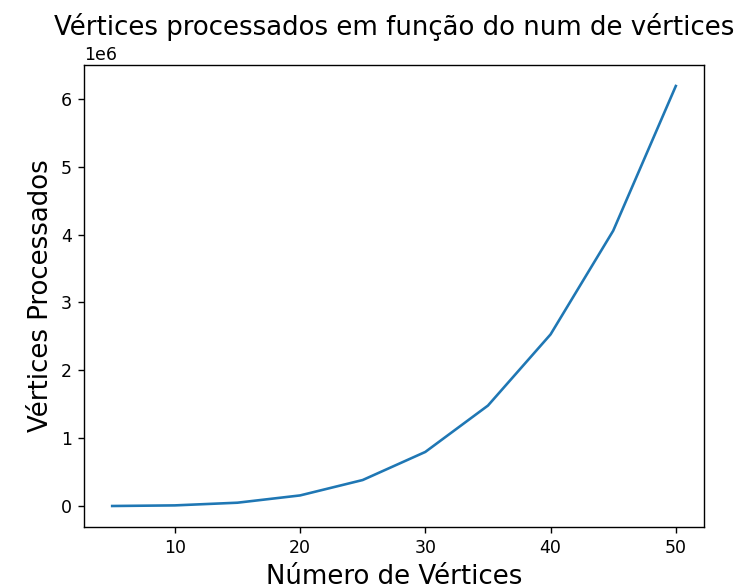
\includegraphics[width=\linewidth]{vertices.png} \caption{Vértices processados} 
        \label{fig:vertices}
    \end{minipage}\hfill 
    \begin{minipage}{0.45\textwidth} 
        \centering 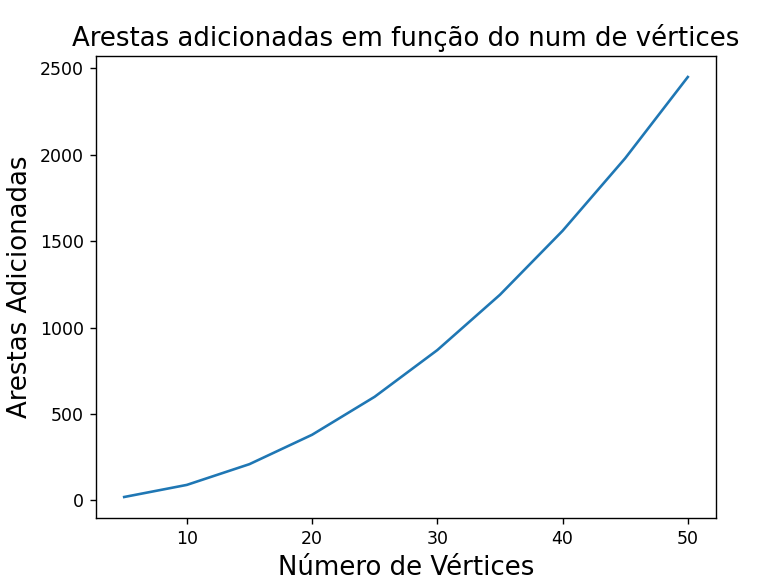
\includegraphics[width=\linewidth]{arestas.png}
        \caption{Arestas adicionadas} 
        \label{fig:arestas} 
    \end{minipage}      
\end{figure}


%-------------------------------------------%
\end{document}